%!TEX root = ../template.tex
%%%%%%%%%%%%%%%%%%%%%%%%%%%%%%%%%%%%%%%%%%%%%%%%%%%%%%%%%%%%%%%%%%%%
%% chapter3.tex
%% NOVA thesis document file
%%
%% Chapter with a short laext tutorial and examples
%%%%%%%%%%%%%%%%%%%%%%%%%%%%%%%%%%%%%%%%%%%%%%%%%%%%%%%%%%%%%%%%%%%%
\chapter{System model and design options}
\label{cha:systemModel_and_designOptions}

In this chapter we present an overview of the system model for our solution. We introduce an architecture model that is able to assure confidentiallity and integrity to the execution of unmodified applications that run sensitive data on cloud computing servers, by leveraging trusted computing tecniques provided by both software and hardware, all according to our adversary model which focus fundamentally on dealing with attackers that can access and read the data during runtime, thus taking value from it. All this without crippling too much the performance levels of the overall system.

In Section \ref{sec:systemModel_overview} we describe a general overview of the system as a whole, introducing the components that make the system. In Section \ref{sec:threatModel_and_securityProperties} we talk about the assumptions kept in mind while creating our solution, as well as defining what is out of our scope.
After that, in Section \ref{sec:systemArchitecture} we go into more details about the components that make part of the whole system, explaining in a fine-grained view how each component works, and what is their purpose in the solution. 
Section \ref{sec:design_tradeoffs} mentions the tradeoffs that our system model faces. We present negative impacts that we expect the technologies we included in our model might add to the system.
In Section \ref{sec:design_openIssues} we take a look into potential problems that we aknowledged our solution's design might induce, and lastly we end with a summary in Section \ref{sec:sysModel_summary}.





\section{System model overview} % (fold)
\label{sec:systemModel_overview}

Our solution can be seen in figure \ref{fig:systemModel}, which is a macro overview of the system. 
The solution we implemented can be divided in two parts - client side and server side - in which the clients interact with the server, which is protected inside a \gls{tee}. 

Although the \textbf{Client} and its purpose is easy to understand - make requests to the server via network - the server its components are more complex. Hereupon, the server is composed by: 
\begin{itemize}
	\item \textbf{Proxy:} Works as an entry point to the whole server-side. It's the component responsible of handling the communication with the Client;
	\item \textbf{Authentication Server:} Authenticates the clients so they can only access the system if they are authorized;
	\item \textbf{Attestation:} Allows the components of the system to prove their identity, thus allowing the rest of the components to treat them as trustworthy;
	\item \textbf{Key-Value Store:} Stores data in-memory. This is the main component we intend to protect, since it is where the information running is held.
\end{itemize} 


All the server components itemized above run on top of trusted hardware (\gls{tee}), inside a third-party cloud server.

\vspace{5mm}
\begin{figure}[htbp]
	\centering
	{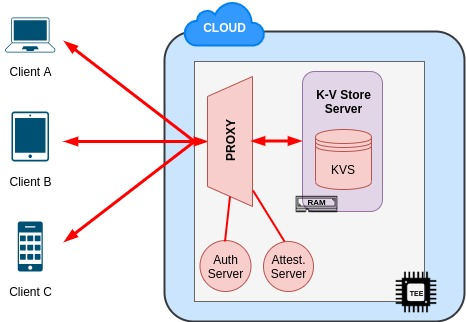
\includegraphics[width=0.7\linewidth]{systemModel}}
	\caption{General overview of the System Model}
	\label{fig:systemModel}
\end{figure}


\section{Threat model and security properties} % (fold)
\label{sec:threatModel_and_securityProperties}

Our solution is designed to offer privacy-enhanced guarantees in protecting data confidentiality, while also ensuring integrity and completeness of results returned to the clients, which we do it by ensuring that sensitive data never runs in plaintext. 
Thus, our system model protects from attackers with intentions of accessing sensitive data and taking advantage and value from it, regardless if the attack is coming from the inside or the outside the host system.


\subsection{Adversarial model definition}

Since the main objective of the solution is to protect data privacy during its execution, we specifically focused on two types of potencial threats: 

\textbf{1-} Users that attack the system and find a way of getting access to high privileges. This is a type of user that can control the system as he pleases, with superuser access, meaning that he will be capable of manipulating the host \gls{os} and other low level privileged components, through which he will manage to access the data running in memory;

\textbf{2-}  Honest-but-curious users, which are users that already have higher privileges, and may or may not have direct access to the hardware. They can snoop easily on private data, since they are considered trusted, so they can read it, learn it and take advantage of it.

We consider to be out of scope denial-of-service attacks, side-channel attacks that exploit timing and page faults.
It is important to refer that with this solution, since we are focusing on using in-memory \gls{kvs}s, our target will not include ensuring confidentiality and integrity to data stored in disk, since we do not resort on persisting the data.

\subsection{Countermeasures for privacy-preservation}

Since our objectives are pointed towards an isolated system capable of offering security
and privacy properties, we depend a lot on isolation techniques to make this possible,
provided by both hardware and software (containers).

We looked at \gls{tee} technologies capable of assuring computation and storage security to our system's data during runtime, although implying in a performance tradeoff. 

In addition, to grant an extra layer of isolation and to ensure privacy to the data in each element of our model, we opted to use containerization as a way to keep them independent and the system modular and scalable, enabling ease in the deployment of software running inside the containers, whether it is an \gls{os}, a library
\gls{os} or even entire applications. Running our system inside containers allows it to be deployed in a very similar way, whether running locally or in cloud, which can be very helpful in the implementation process. 





\section{System Architecture}
\label{sec:systemArchitecture}
In this section, we dive into more detail about the components that make part of the system and what purpose do they have in the solution.  

Our solution, which is based on the system model introduced in Section \ref{sec:systemModel_overview}, and as it has been there referred, can be divided into two parts, one part being the Client-side, responsible for making requests to the system, and other being the server, that deals with the execution and storage of the data.

For the Client-side, we only considered them to be benchmark applications and not entire web applications, with only the intent to evaluate the system for our experimental analysis shown later on this dissertation. Thus, we assume that the client is trusted, as long as he can authenticate himself in the system.

As for the server, our goal is to provide privacy to sensitive data running on top of trusted technology - \gls{tee}s - without crippling too much the performance levels of the application running. 
Hereupon, our server-side, which we run inside a Cloud server, can itself be divided into multiple components: a Proxy, an Authentication Server, an Attestation component and a \gls{kvs} component. All these are running inside containers on top of a \gls{tee}, more specifically Intel-\gls{sgx}.

According to what we have already studied, to run applications on top a \gls{tee} usually causes the system to take a performance penalty. To mitigate those penalties, we included additional layers of technology, frameworks specifically designed to work with these trusted technologies and to soften the performance impact \gls{tee}s have on applications that leverage their properties. 

\subsection{Client-Side Operations}

For the client-side, as mentioned in the beginning of this section, we only considered benchmark clients. We use these benchmarks to evaluate the system by making simple requests to the Proxy, while calculating metrics that we found essential to use in our pratical evaluation of the solution, in order to validate the full-fledged conditions in supporting the \gls{kvs} REDIS. And as long as the user is registered in the authentication server, it is considered trusted.

To start a communication with the server, a client: 

\textbf{1.} Reaches the authentication server to authenticate itself;

\textbf{2.} Interacts with the proxy after being granted authorization to do so, as long as the authorization is valid, as we can observe in the figure \ref{fig:client_serverModel}. 

All this communication process is secured through TLS over HTTP.

\begin{figure}[htbp]
	\centering
	{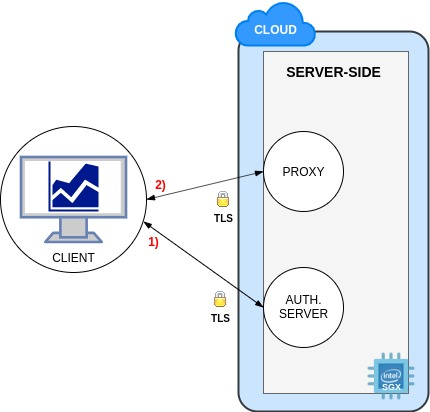
\includegraphics[width=0.5\linewidth]{comm_client_server}}
	\caption{Communication between client and server}
	\label{fig:client_serverModel}
\end{figure}



\subsection{SGX-Enabled REDIS solution} % (fold)

The server runs on top of a \gls{tee}, that being Intel-\gls{sgx}. As we studied, applications can't simply be placed on top of a \gls{tee}, in this case \gls{sgx}, and expect them to perform as efficiently as they do without this extra layer of security. 
Since \gls{sgx} completely isolates what is running inside its enclaves from the rest, even from the \gls{os}, it cripples the performance of the system for multiple reasons. Everytime a system call needs to be performed by running code, the thread of execution needs to leave the enclave to execute it. Only after it has completed executing the system call, the thread can come back inside the enclave. This process takes a lot of effort for the system, since it envolves a lot of encryption functions to take place. 
Also, since enclaves are small in-memory regions (size depends on the hardware used), when running a normal or large sized application on top of \gls{sgx} it usually means that the code does not fit all at once inside the \gls{epc}. 
Thus, parts of the application need to leave the enclave in order to fit the other parts that are needed at that time, resulting in a lot of encryption and decryption taking place due to page swapping between the \gls{epc} and the rest of the memory, in order to keep the integrity of the data.  

Hence, we opted to use SCONE, which we covered in Section  \ref{ssec:scone}, as a way to better leverage \gls{sgx} properties. It allows us to run the server components mentioned before on containers capable of running applications inside \gls{sgx} enclaves with effectiveness. This happens mainly because SCONE containers include a small library of system calls that can be accessed statically inside the enclave. Also it supports asynchronous system calls, meaning that when dealing with the need to execute a system call outside the enclave, SCONE switches the execution thread to one running outside the \gls{epc}, avoiding the performance penalty caused by the need for a thread to exit the enclave. 

Thus, we mitigate some of the downsides of the usage of \gls{sgx}, so that the following components that are part of the system can leverage \gls{sgx}s security properties with ease:

\vspace{5mm} 

\textbf{1) Proxy -}
Although it is an extra layer of overhead, we thought the addition of a Proxy component to be a worthy investiment because it is designed to serve multiple purposes. 
First of all, we use it as a gateway for the system to communicate with the outside. It acts as a single point of access, enabling the rest of the system to scale, adding no extra complexity to the client-side. By having a Proxy, everything the client has to do is to reach the Proxy itself, while the logic regarding the redirection to the correct server instance that will manage the client request will be done by the Proxy. Adding to that, it allows the system to only need a single firewall, instead of configuring one for each KVS instance.

The proxy is also the responsible for only allowing authenticated clients to access the system, through interactions with the authentication server. 

\vspace{5mm} 

\textbf{2) Authentication Server -}
We added an authentication component responsible for authenticating every client that wants to interact with the system, by assigning access tokens to those allowed, which the clients will then use to communicate with the system after the Proxy validates them.
 
Although some \gls{kvs}s (i.e., Redis) have the possibility to configure authentication for each replica, we believe that option would add an extreme layer of complexity that we do not want, due to the fact that each replica needs to be configured individually. Therefore, if we use a cluster of \gls{kvs} instances and begin to scale their number, the complexity of that task everytime a new user is being granted permission to access the system will be huge. Thus, by including a server designed only to deal with the authentication process, the configuration only needs to happen once for the system to know which users are allowed.

\vspace{3mm}

\begin{figure}[htbp]
	\centering
	{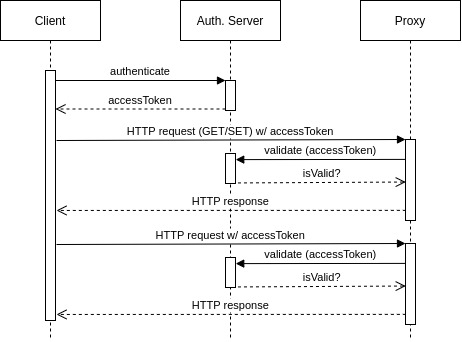
\includegraphics[width=0.9\linewidth]{authSeqDiagram}}
	\caption{Authentication Process}
	\label{fig:authProcess}
\end{figure}

In figure \ref{fig:authProcess} we see that in the first interaction with the system, the Client reaches the Authentication Server in order to get an access token to use as proof of authentication in its future requests. This token is valid for only a certain period of time. After it has expired, the Client needs to reach the Authentication Server again, in order to get a new valid token. While the token is valid, the Client can make requests to the server-side by interacting with the Proxy. The Proxy then validates the token and only if it is indeed valid will the Proxy process the Client request.

\vspace{5mm} 

\textbf{3) Attestation -}
For the component accountable to deal with attestation for the system, we follow a remote attestation policy where a remote system is the one who holds the defined secrets and provides them to the system components when they successfully attest themselves to this remote server.

As we mentioned earlier, we resort on SCONE as a way to run our components inside \gls{sgx}. SCONE also offers a mechanism to attest the enclaves where SCONE containers are running the applications, which we use to add the attestation property to our system. 

SCONE's attestation mechanism, called SCONE Configuration and Attestation Service (or CAS) \cite{sconeCAS}, consists on exposing a remote component provided by SCONE itself that manages the secrets (i.e., keys) of an application, to whom enclaves will then try to prove their identity in order to access those secrets, so they can execute their designated application. 

In CAS we define each application access policy, reflecting which enclave have permission to execute them. The confidentiality and integrity of this policies and their secrets are ensured by CAS itself. To modify and read a policy, the client (in this case, us) needs to have knowledge of the private key that pairs with a public key, which is stated in the policy itself upon creation. Thus, no admin managing CAS can read or modify the policies defined remotely.

For an application to prove their identity to CAS, and thus get access to the secrets, it needs to be attested locally so it gets the attestation key involved - a key pair that CAS shares with a local component so they can validate each other's involvement. The key is then recognized by CAS and the attestation is considered valid (although no access to the secrets is given yet). With that in mind, SCONE's attestation mechanism adds a second component, which runs locally inside the system environment. Local Attestation Service (or LAS) receives attestation requests by the enclaves that intend to attest themselves to CAS, and signs them with the attestation key, creating a quote that can be verified by CAS. After getting this quote, any enclave can reach the CAS to try and access the secrets to run the application, but only if they are allowed by its defined policy. This completes the attestation process of an application running in an \gls{sgx} enclave. 

\begin{figure}[htbp]
	\centering
	{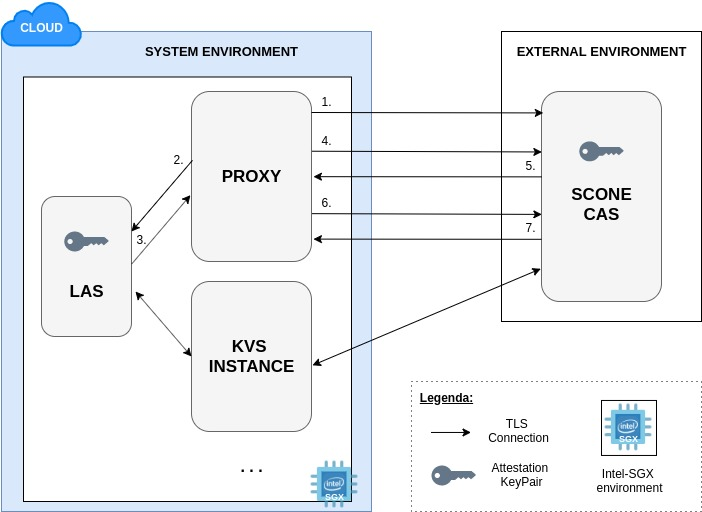
\includegraphics[width=0.6\linewidth]{attestationModel}}
	\caption{Attestation Model}
	\label{fig:attestationModel}
\end{figure}

In Figure \ref{fig:attestationModel} we present a visual display of the attestation process described above, taking place inside our system model.

The attestation starts with the enclave of an application (i.g., the Proxy component of our system) establishing a HTTPS connection with the remote component CAS endpoint. Afterwards, the enclave requests the attestation from LAS, which will then sign a message with the attestation secret key, resulting in a Quote. The Quote is then used by the enclave to validate its own attestation with the help of CAS. After validation, the enclave requests access to the secrets defined in the policies that CAS helds. If the enclaves is indeed specified to run the referred application it intends to run, CAS shares the secrets, thus completing the attestation process with success. In Figure \ref{fig:attestationProcess} we present a diagram with the steps just described.

\begin{figure}[htbp]
	\centering
	{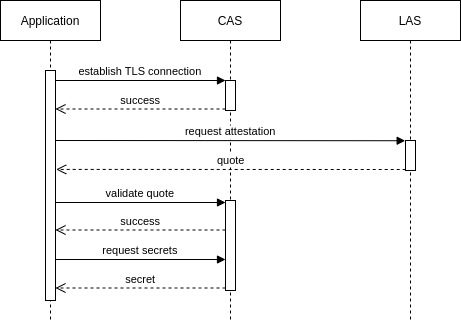
\includegraphics[width=0.8\linewidth]{attestDiagram}}
	\caption{Attestation Process}
	\label{fig:attestationProcess}
\end{figure}


\vspace{5mm} 

\textbf{4) Key-Value Store -}
For the \gls{kvs} component, we use the Redis \gls{kvs} that can be used with different configurations, offering multiple strenghts to the execution and storage of data, especially if run in Cluster mode, offering scalability, fault-tolerance and eventual consistency of data, in some cases without even resulting in any overhead. 
If each replica of the cluster is set to run in independent machines, the majority of the complexity is handled by the network, allowing the performance levels to match the values obtained by a single instance Redis while still offering all the properties mentioned above. Redis supports different configurations: 

\textbf{Standalone.} The simplest configuration that a Redis instance can run in. It offers the properties of a single Redis database. It is very simple, very stable and easy to maintain.

\textbf{Master-Slave.} Offers replication and eventual consistency of data, with writes only possible in the Master node, and read-only Slave nodes.

\textbf{Cluster.} Although it is the most complex configuration, beyond replication and consistency, it also adds huge scalability possibilities to the system. It also considers Slave nodes to be read-only.

In our solution we deploy Redis instances capable of running in all the configurations mentioned - Standalone mode, Master-Slave and Cluster - as a way to test the behavior of the system in each of those configurations. It is also important to note that each Redis replica runs inside its own container, regardless the configuration it was set to run in. 

\vspace{5mm}

\begin{figure}[htbp]
	\centering
	{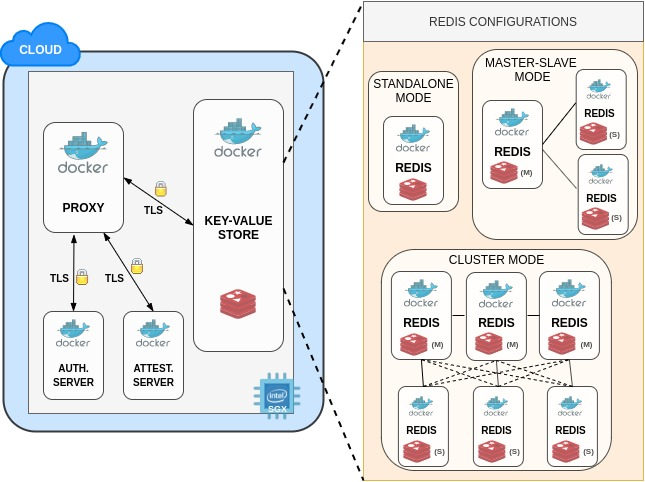
\includegraphics[width=0.7\linewidth]{systemWithMoreContext}}
	\caption{Server-side overview of the solution}
	\label{fig:serverside_systemModel}
\end{figure}

\vspace{5mm}
All the communications between the components that make up the server-side are secured by TLS over HTTP, as a way to keep confidentiality of the data during communications all over the system. The access to this TLS libraries inside \gls{sgx} is possible due to the inclusion of openSSL on the static library that SCONE containers offer. By having openSSL statically inside the enclave, no tangible overhead is added to the system, since the execution doesn't need to switch to a thread outside the enclave, in order to respond to the system call, thus establishing a HTTPS connection directly from inside the enclave. 

  
\section{System Model Design Tradeoffs}
\label{sec:design_tradeoffs}

Although our system model focus on assuring confidentiality and integrity to application data running inside a third party system, by leveraging trusted computation techniques, this comes at a cost. Tradeoffs have to take place, particularly between security and performance, where more security usually means less performance. 
Thus, the usage of this trusted techniques are not always considered worthy, alongside the fact that the levels of isolation they assure can also mean less fluidity for the system in general.  

\gls{tee}s give the system extra levels of security during the execution of data by isolating the code from the rest of the system, even from the high privileged components. This isolation is either given by encrypting a \gls{vm} in which the code is executing, or encrypting only the region of memory dedicated to run the code. 

In our system model, \gls{sgx} works alongside the second option, encrypting the enclave memory region dedicated to the application, while also trying to keep the \gls{tcb} as small as possible, by limiting the functions supported inside the enclave as a way to increase the level of security. 
This leads to a tradeoff, since less supported functions inside the enclave means that the thread of execution will more likely need to leave the enclave in order to execute system calls, or other kind of essential operations, resulting in major overheads due to all the encryption involved. This has a big performance impact when dealing, i.e., with network-heavy services, which usually have a high system call frequency.

Also, by only relying on the encryption of the enclave memory region, \gls{sgx} encounters problems when confronted with applications that are bigger than the enclave itself (keep in mind that an enclave size is usually really small, only around 64MB and 128MB \cite{sconePaper}). 
When the memory space needed for the application is bigger than the enclave size, page swaps between the enclaves \gls{epc} and the untrusted memory take place, through a mechanism provided by \gls{sgx}. Since this scenario envolves a lot of encryption and decryption to happen, it induces the system into huge performance overheads.

SCONE, along with some other recent technologies, has been referred as a possibility to help mitigate some of those performance losses. 
It does it by: 
1) trying to level the scale between the two factors, security and performance, and
2) maximizing the time threads spend inside the enclave.
The first factor due to keeping the \gls{tcb} as small as possible, but with enough functionalities to allow the system to perform with efficiency. As mentioned before, SCONE containers include a small (and trusted) library with system functionalities that can be used inside the enclave. It increases the \gls{tcb} in a controlled way, while improving the performance levels and fluidity of the system.
And the second factor by allowing asynchronous system calls. This enables the possibility to swap the execution from inside the enclave to a thread outside whenever a system call left out of the \gls{tcb} is needed, thus avoiding threads to exit the enclave.

However, even helping soften some of the tradeoffs related to using trusted technology to run our system model, using SCONE doesn't make our solution perfect. Thus, we still expect to observe security and performance tradeoffs, however we are confident those to be way less expressive with the help of SCONE.

% section importing_images (end)
\section{Open Design Issues} % (fold)
\label{sec:design_openIssues}

Looking back at our model, we can think that the whole availability of the system depends highly on the single proxy instance working as entry-point for the whole system, and so all can be compromised if it fails to work. 
Replication of the proxy instance can be seen as a measure to mitigate this problem, and although this is doable, we considered it to be out of scope for what we choose to evaluate in this thesis. 



\section{Summary} % (fold)
\label{sec:sysModel_summary}

We designed our model with the objective to grant integrity and confidentiality to applications with data running inside a cloud host. With that in mind, we focus on finding a solution that enables the use of a \gls{tee}, in this particular case Intel-\gls{sgx}, while still assuring good performance to the system. 
For that, we adopted SCONE as a mediator between the application and the trusted hardware. SCONE is a secured Linux container that can be used to deploy entire applications with ease on top of \gls{sgx}, and allows better performance levels when running applications on trusted hardware, due to the inclusion of a static small library of system calls directly inside the container, thus minimizing the number of times enclave exits need to happen because of a system call that is not allowed inside the \gls{epc}. This is a huge factor since it is considered a major performance dropper on applications running with \gls{sgx}. 
With SCONE we are able to deploy various configurations of Redis \gls{kvs} on top of \gls{sgx} with relative ease, allowing us to assure our initial objectives:  grant integrity and confidentiality to the data running and being stored in-memory. 
As for the communication process, to better protect the system, we implemented a Proxy server. It serves as a gateway to the entire system, and it's responsible to validate the authentication of the clients, which is granted by an Authentication Server. Lastly, we use an Attestation Server responsible for attesting all the components running in the system. To note that all this  components run on top of \gls{sgx} with the help of SCONE. 

Also, by protecting each communication link, either between client and server or between the server components themselves, with TLS, we can assume that our system complies to the adversary model defined.

In the next chapter, we will show how we implemented the prototype for the system model discussed here.

% \subsection{Inserting Figures Wrapped with text} % (fold)
% \label{ssec:inserting_images_wrapped_with_text}
% 
% You should only use this feature is \emph{really} necessary. This means, you have a very small image, that will look lonely just with text above and below.
% 
% In this case, you must use the \verb!wrapfiure! package.  To use \verb!wrapfig!, you must first add this to the preamble:
% 
% \begin{wrapfigure}{l}{2.5cm}
%   \centering
%     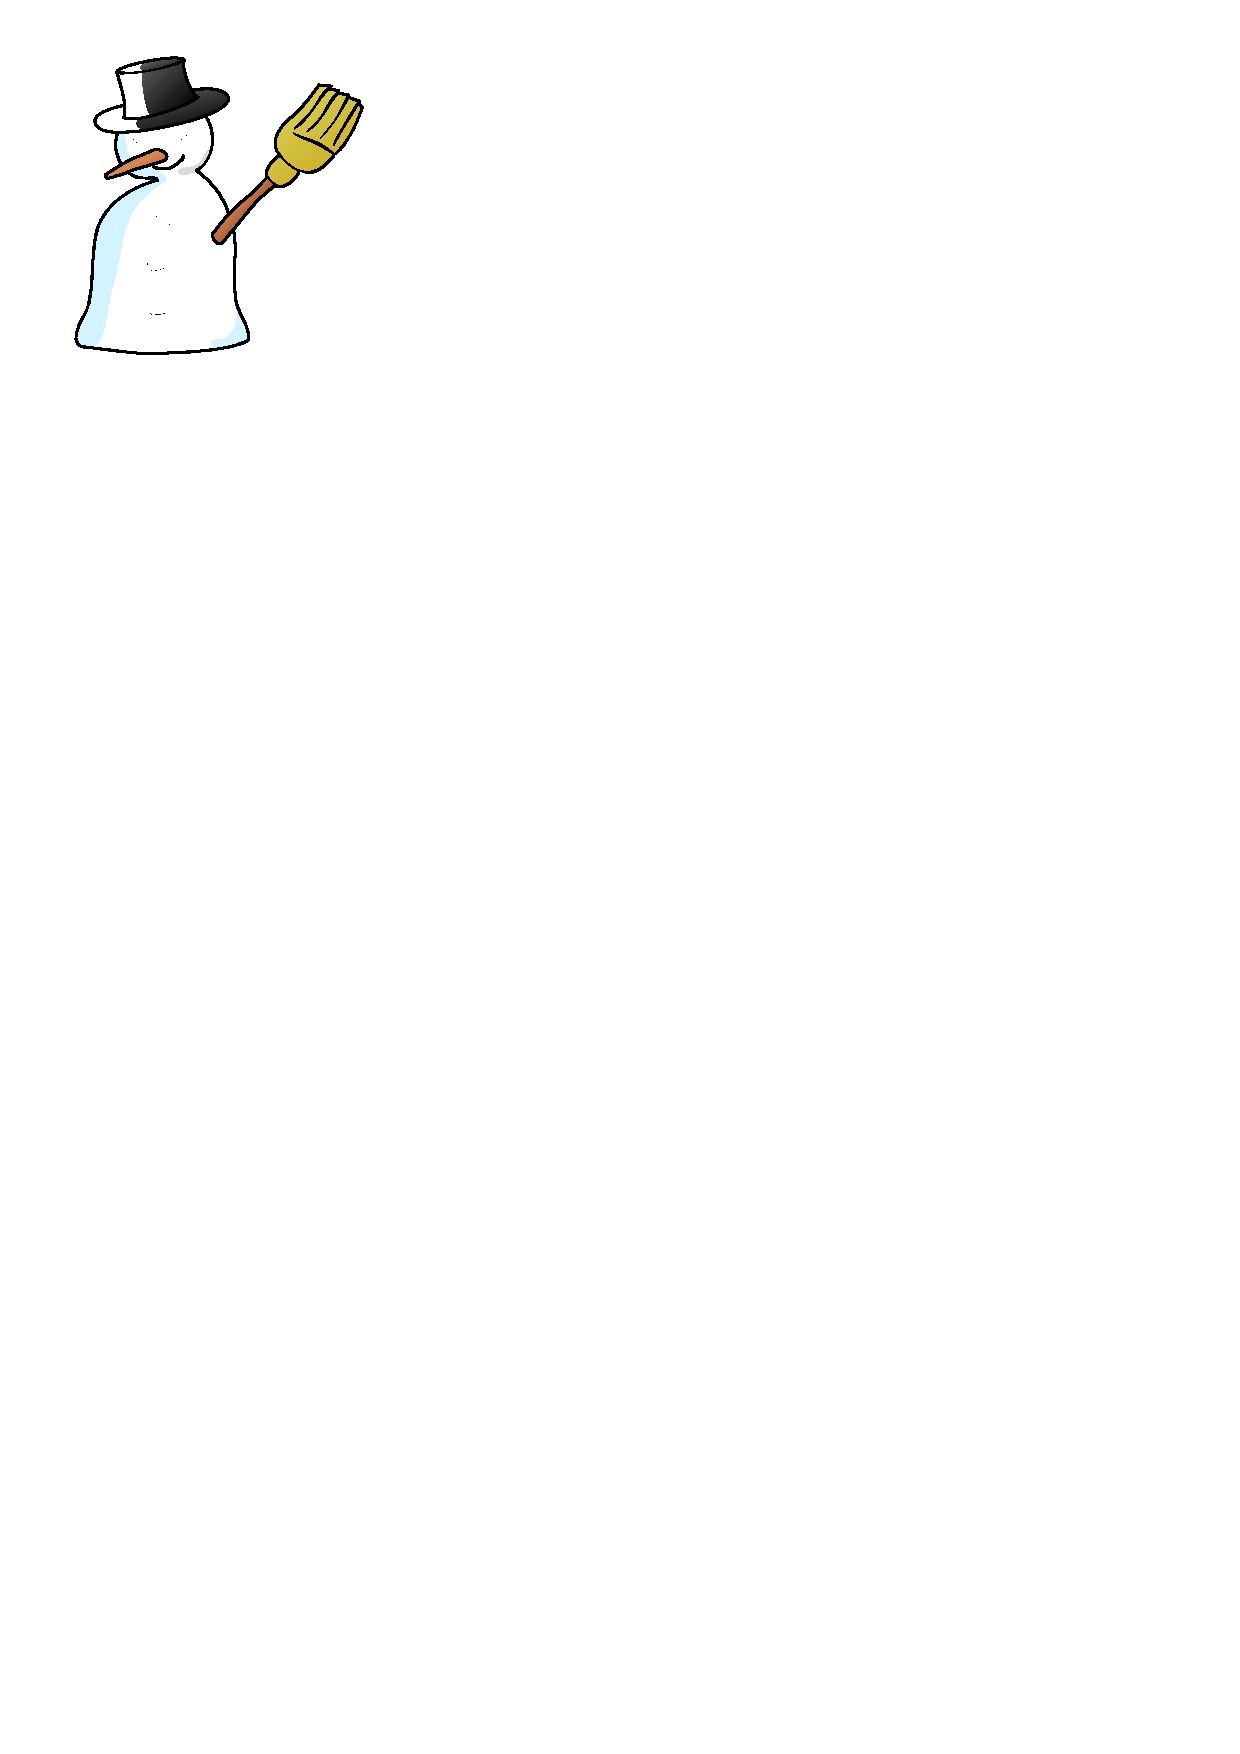
\includegraphics[width=2cm]{snowman-vectorial}
%   \caption{A snow-man}
% \end{wrapfigure}	
% 
% \noindent\verb!\usepackage{wrapfig}!\\
% This then gives you access to:\\
% \verb!\begin{wrapfigure}[lineheight]{alignment}{width}!\\
% Alignment can normally be either ``l'' for left, or ``r'' for right. Lowercase ``l'' or ``r'' forces the figure to start precisely where specified (and may cause it to run over page breaks), while capital ``L'' or ``R'' allows the figure to float. If you defined your document as twosided, the alignment can also be ``i'' for inside or ``o'' for outside, as well as ``I'' or ``O''. The width is obviously the width of the figure. The example above was introduced with:
% \lstset{language=TeX, morekeywords={\begin,\includegraphics,\caption}, caption=Wrapfig Example, label=lst:latex_example}
% \begin{lstlisting}
% 	\begin{wrapfigure}{l}{2.5cm}
% 	  \centering
% 	    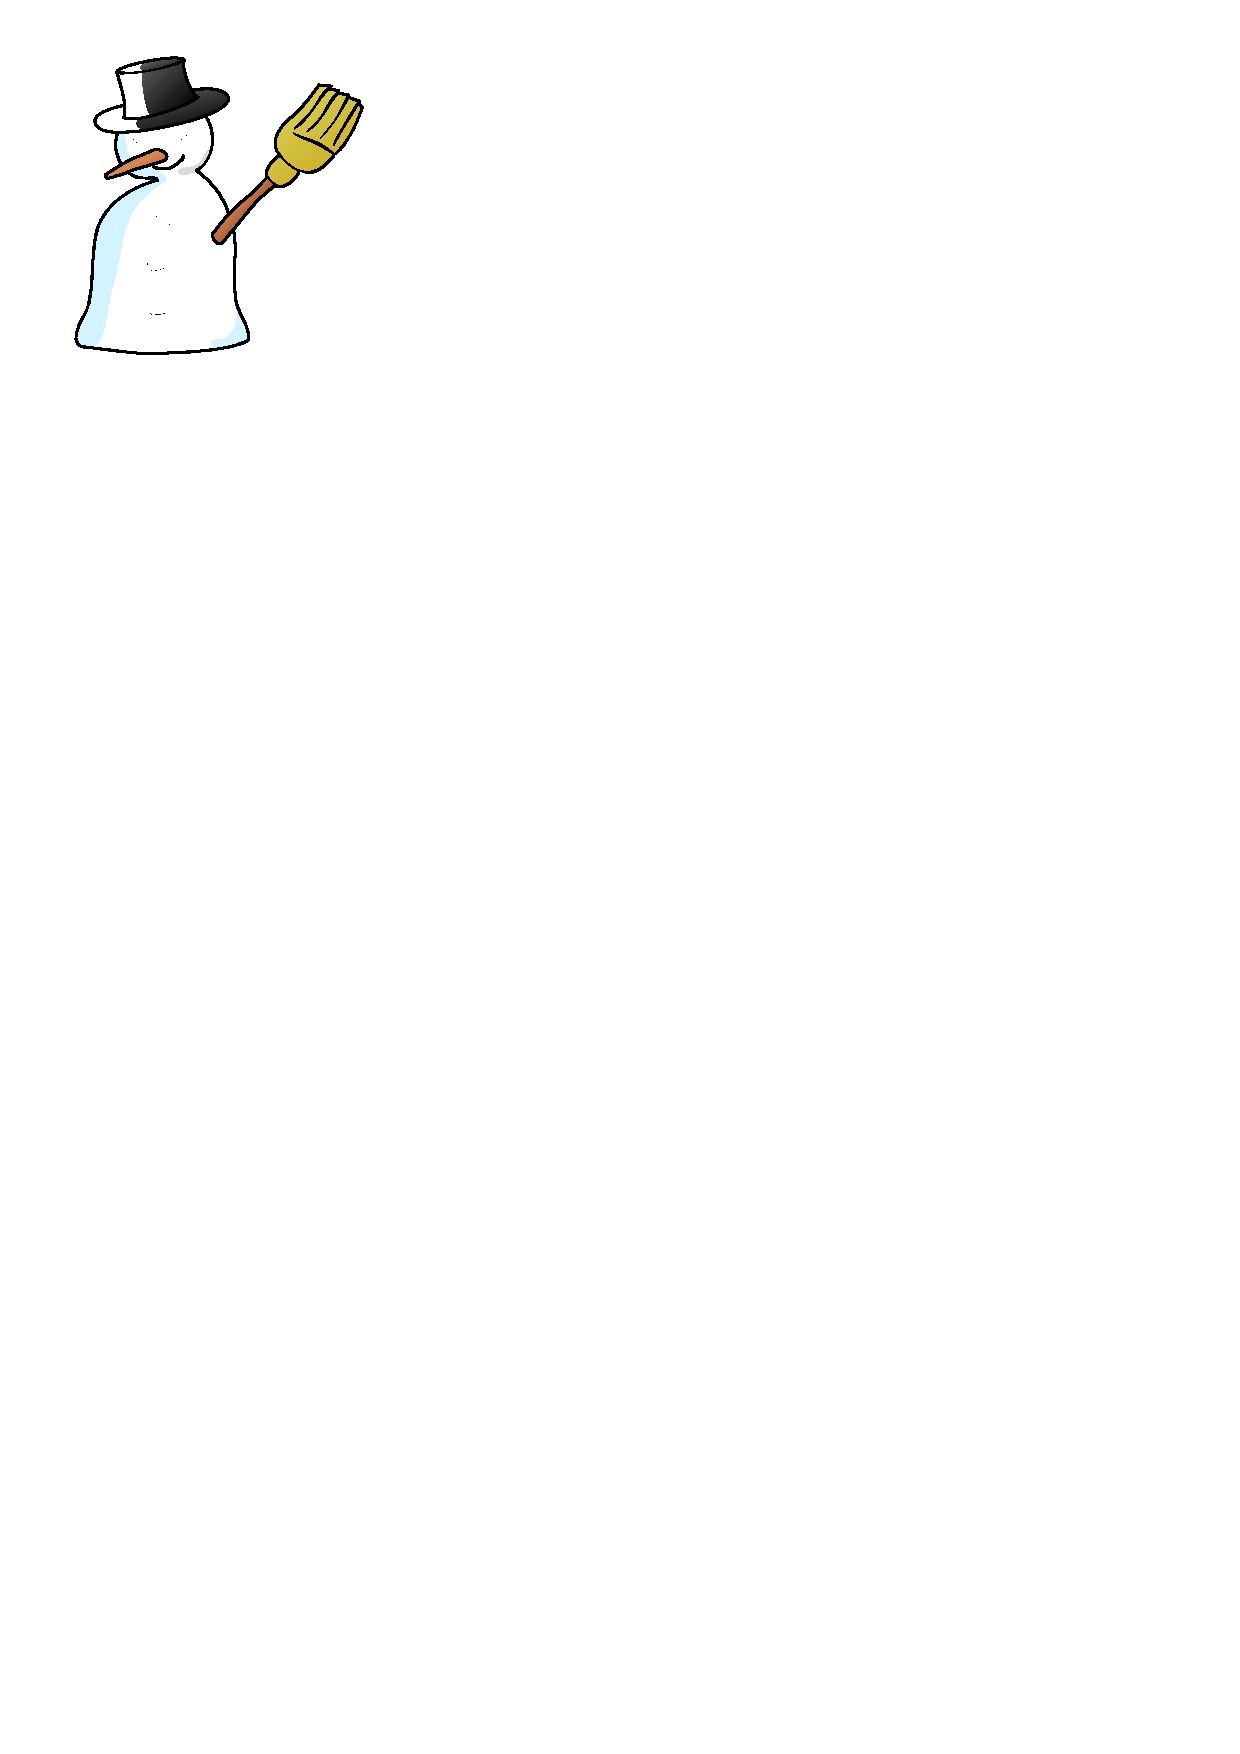
\includegraphics[width=2cm]{snowman-vectorial}
% 	  \caption{A snow-man}
% 	\end{wrapfigure}	
% \end{lstlisting}

% subsection inserting_images_wrapped_with_text (end)

% section floats_figures_and_captions (end)

